\section{电磁铁}\label{sec:10-5}

我们知道,通电的螺线管具有磁性。通电螺线管磁性的强弱跟哪些因崇有关呢?
这个问题让我们通过实验来解答。

如图 \ref{fig:10-28} 所示,给螺线管通电,铁块受到螺线管的吸引使弹簧伸长。
调节变阻器,改变通过螺线管的电流强度,可以看到,电流越强,弹簧被拉伸得越长。
这表明通过螺线管的电流越强,它的磁性也越强。
如果换用匝数不同的螺线管而保持通过螺线管的电流强度跟前面的实验一样,
可以看到,螺线管的匝数越多,弹簧被拉伸得越长。
这表明通电螺线管的匝数越多,它的磁性也越强。

\begin{figure}[htbp]
    \centering
    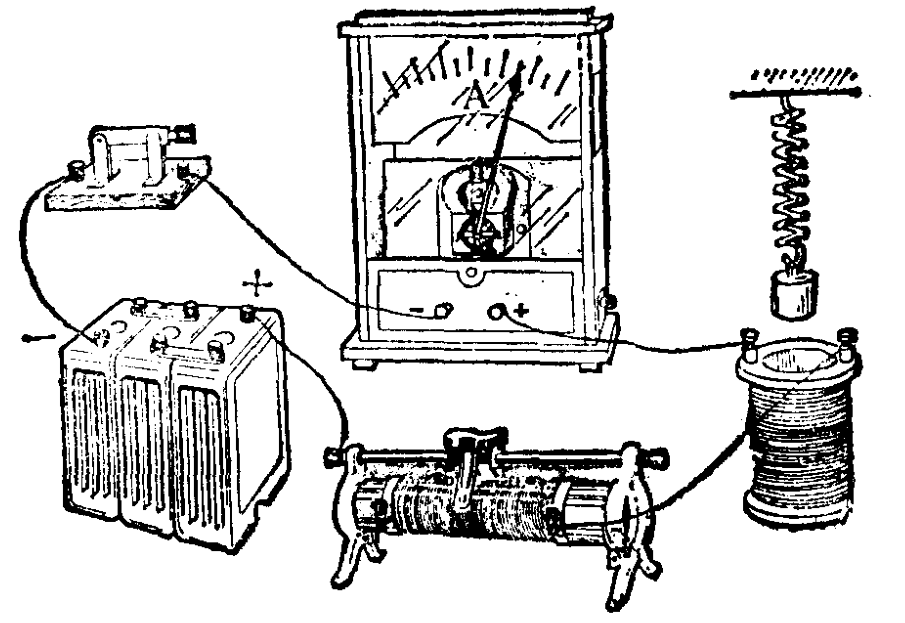
\includegraphics[width=0.7\textwidth]{../pic/czwl2-ch10-28}
    \caption{研究通电螺线管的磁性}\label{fig:10-28}
\end{figure}

在图 \ref{fig:10-28} 的实验里,如果不改变通电螺线管的电流强度,
而将铁棒插入螺线管中,可以看到,弹簧显著伸长。
这是由于铁棒在通电螺线管中被磁化也有了磁性,铁块受到通电螺线管的磁场和被磁化了的铁棒的磁场的共同作用。
因此,插入铁棒后螺线管的磁场大大增强。人们利用通电螺线管的这个特性制成了电磁铁。
内部带铁心的螺线管叫做电磁铁。常用的电磁铁大都做成 U 形,目的是让它的两个磁极同时吸引物体,使吸引力更强。

电磁铁有很多优点:它的磁性有无可以由通断电来控制,它的磁性强弱可以由电流的强弱来控制,
它的南北极可以由变换电流方向来控制,使用起来很方便。因此在生产、生活、科学技术上用得很多。
例如,电磁起重机上有一块大的电磁铁,通上电流,一次能把几吨钢材吸起来搬运到指定的地方去。
电磁选矿机靠电磁铁的作用能把铁和非铁物质分开(图 \ref{fig:10-29})。
此外,在电铃、电报机、电动机、发电机、自动控制上都应用了电磁铁。

\begin{figure}[htbp]
    \centering
    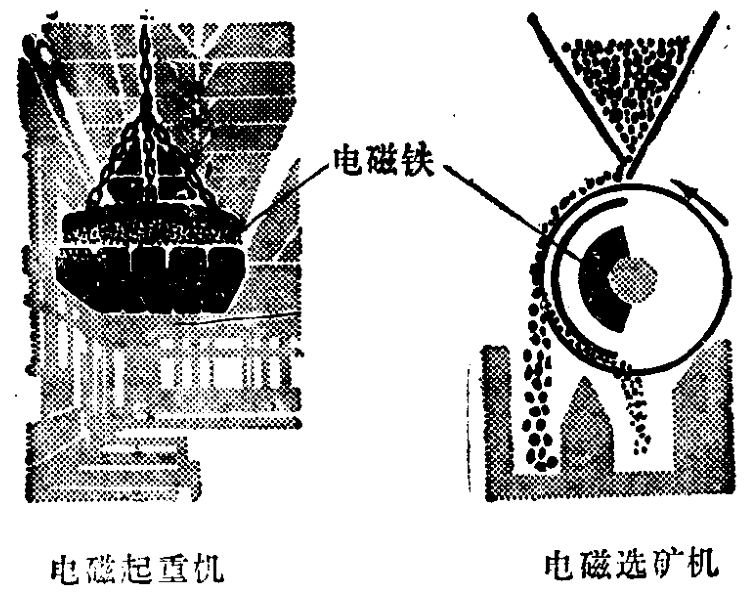
\includegraphics[width=0.6\textwidth]{../pic/czwl2-ch10-29}
    \caption{}\label{fig:10-29}
\end{figure}


